\documentclass[man,noapacite]{apa2}
\usepackage{apacite2}
\usepackage{graphicx}

\title{Problems of statistical power in infancy research}

\author{Michael C. Frank}
\affiliation{Department of Psychology, Stanford University}

\abstract{Reproducibility is a core value for empirical research, but there is increasing concern throughout psychology that weak statistical standards and methodological practices have led to low empirical rates of replication. Because research with infants is labor-intensive and slow, reproducibility rates have not been assessed directly. Yet the small sample sizes and limited numbers of measurements available in this work lead to significant concern about this field. I show here that much published infancy research is likely to be underpowered and that the conventional sample sizes are insufficient for detecting the majority of effects, especially when post-hoc analyses are employed. I describe a set of best practices for infancy research that may mitigate some of these issues, and present a simple tool for power analysis.}

\shorttitle{Infancy methods}
\rightheader{Infancy methods}

\acknowledgements{This work supported by a John Merck Scholars Fellowship. Thanks to ...

~

\noindent Please address correspondence to Michael C. Frank, Department of Psychology, Stanford University, 450 Serra Mall (Jordan Hall), Stanford, CA, 94305, tel: (650) 724-4003, email: \texttt{mcfrank@stanford.edu}.}


\begin{document}
\maketitle                            

\section{Introduction} 

Replicability is a cornerstone of empirical science. If an experiment cannot be repeated, it cannot be built on by future work, and its theoretical value is limited at best. 




The issues with questionable research practices, statistical power, and null-hypothesis statistical testing more broadly are well-known at this point, and my goal here is not to reiterate these discussions. Interested readers are directed to \citeA{simonsohn2011}, \citeA{cumming2013} etc. for tutorial discussion. In the current article, my goal is to focus specifically on the infancy literature---even more specifically on looking time studies---and highlight a number of methodological practices that may lead to a particular inflation of false positives in this literature. 

I should note that although I recognize the issues with the null-hypothesis significance testing framwork, I believe it is

\section{Issues specific to infancy research}


\begin{enumerate}
\item Sample sizes
\item 
\end{enumerate}

\section{Systematic literature review}

\paragraph{Coding protocol}

Age group
study
type of statistical test
p value
effect size (if possible)
mediation/post-hoc analyses?

\paragraph{Results}



\section{Statistical power: Simulations}

Statistical power is the probability that a particular statistical test will reject the null hypothesis. 

I show simulations here that demonstrate issues with negative control groups, the use of post-hoc mediator variables

\subsection{Basic power analysis}

The key question of course for basic power analysis is the effect size that you would like to detect. If effects are large, then small samples are more justified. If effects are smaller, then small samples inflate the risk of false positives

\subsection{Negative control groups}

A common practice in infancy research is the addition of negative control experiments---that is, control groups that test an alternative explanation and for which the prediction is a failure. It is not unknown to see these control groups presented as distinct studies, with independent statistical tests performed. Then, a positive result in the primary experiment of interest and a failure to find a statistically significant result are used together to argue for the importance of the factor that was manipulated in the first experiment. 

Of course, this experimental logic is not sound. These two experiments are in fact \emph{different conditions} of the \emph{same experiment}, because there is a manipulation whose causal importance is being assessed by the contrast in effects between groups. And since these two conditions are being compared, the difference between them must be tested statistically. The alternative strategy of 
\cite{gelman,nrn-significnotsignif}

\begin{figure}[t]
\centering
  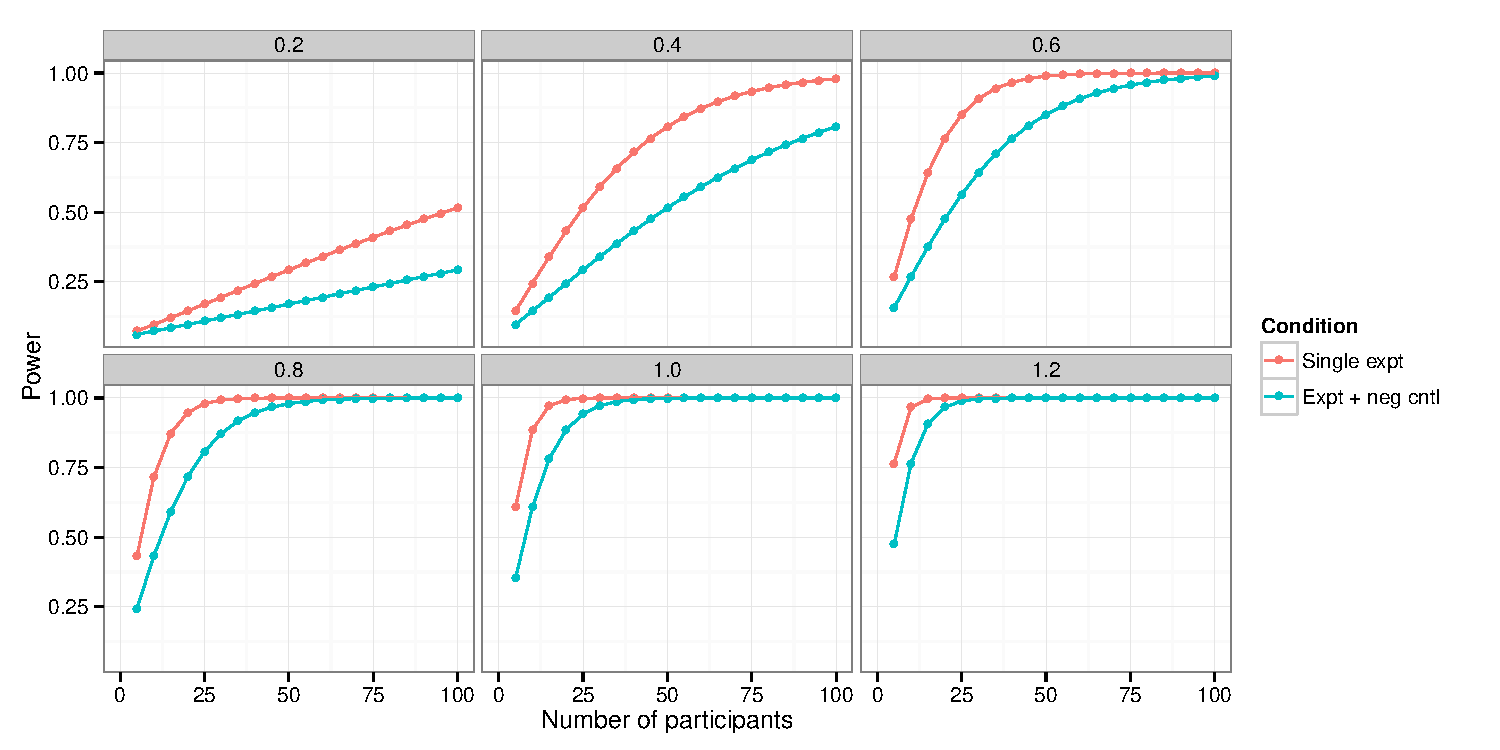
\includegraphics[width=6.5in]{../plots/power_gap.pdf}
	\caption{\label{fig:powergap} .... }
\end{figure}

\subsection{Moderation, mediation, and other post-hoc analyses}

\begin{figure}[t]
\centering
  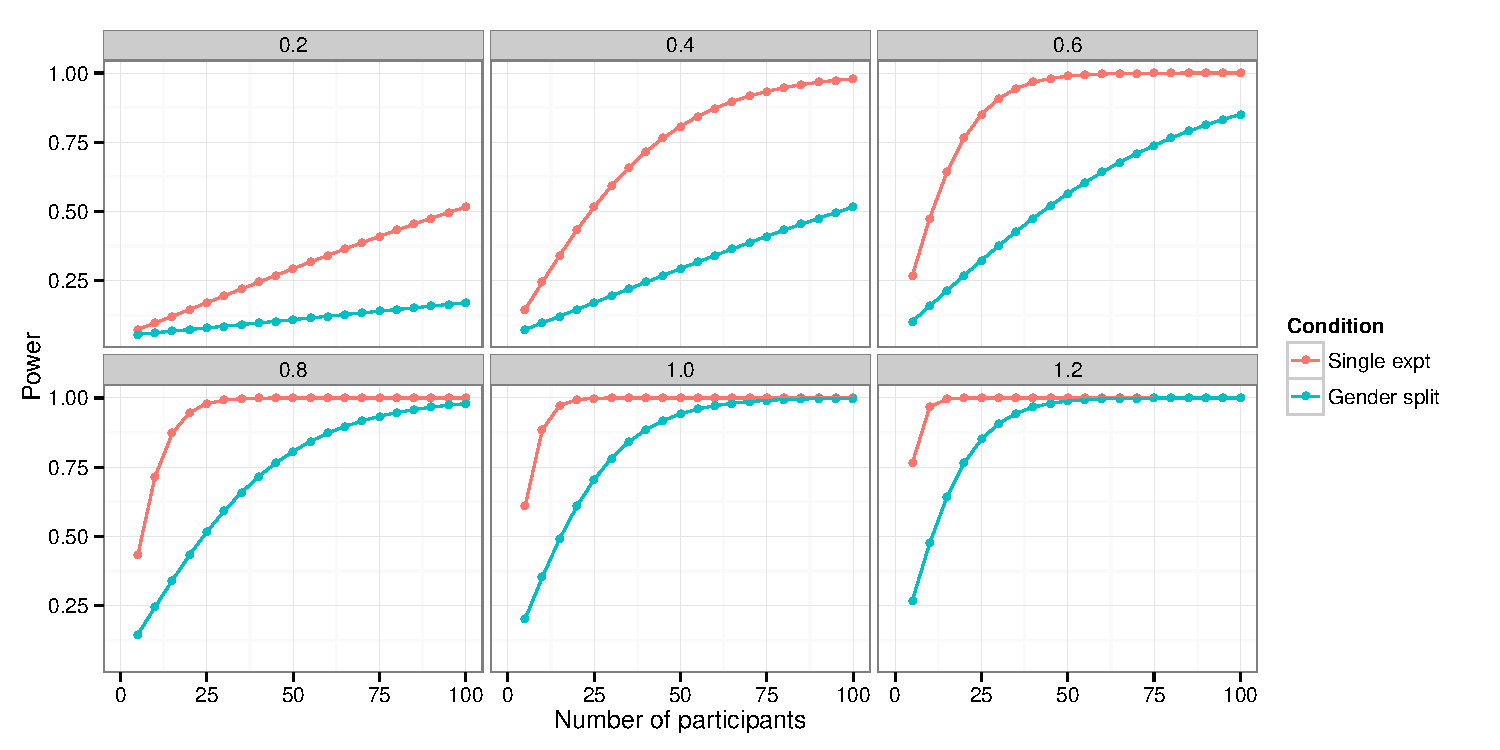
\includegraphics[width=6.5in]{../plots/post_hoc.pdf}
	\caption{\label{fig:gender} .... }
\end{figure}

Consider a researcher who runs a standard infancy study with N=16 or N=24 and then goes on to explore a gender effect within that dataset. Even if 

Figure \ref{fig:gender} shows the results of a power analysis that assumes that the gender effect is equal in magnitude to the original effect (essentially, that one gender showed the predicted effect and the other showed zero effect). Even if the original effect was very well-powered, the power to detect the gender effect is very small. Consider a case with $d=.8$, a large effect, and $N=20$: the power on the original study is .95: more than sufficient. But the power to detect a gender effect is .43. 

There are two reasons for this asymmetry. The first is that by considering a moderator of the effect like gender, the researcher is considering a between-subjects, rather than a with-subjects, measure. Such measures are always more variable. The second is that by considering this between-subjects measure, the researcher has reduced the effective sample size in each group to 8 infants. Considered this way, it's hardly surprising that the power to detect 

Finally, as has been noted prominently before, the post-hoc, data-contingent exploration of mediator and moderator variables increases the false-positive rate, due to issues of multiple comparison  \cite{simonsohn2011}. Even if researchers report these as subsidiary analyses that do not compromise the main analysis, there is nevertheless a larger chance that such subsidiary analyses are false. 

To illustrate this pattern, consider the 

\section{Recommendations}

We close with a number of recommendations
These are: 1) larger samples, 2) internal replications (especially including developmental replicates), 3) use of more transparent visualizations, 4) avoidance of post-hoc analysis, and 5) use of multi-trial paradigms.

\paragraph{Internal replications}

The strongest test of the reproducibility of a finding is a direct replication. Authors should be encouraged to perform and report such replications in their manuscripts, and reviewers should feel empowered to request them. Authors

One 
 
Developmental replicates

\paragraph{Larger samples}

As is evidence from the preceding discussion, sample sizes in 

Power analysis can be a helpful guide

In sum, the number of participants for a study will likely vary widely from study to study, but it will rarely be 16. 



\paragraph{Visualization}


\begin{figure}[t]
\centering
  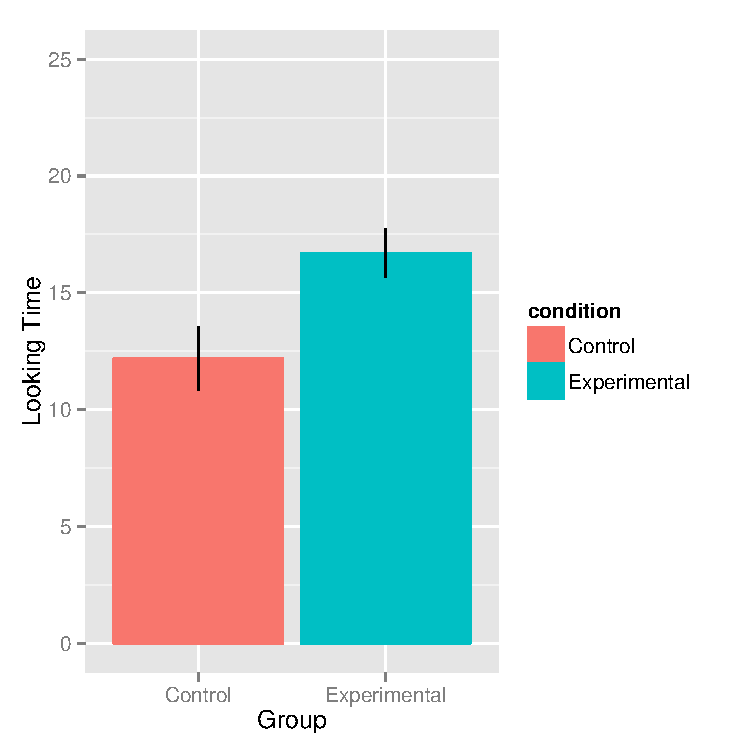
\includegraphics[width=2.5in]{../plots/bars.pdf}
  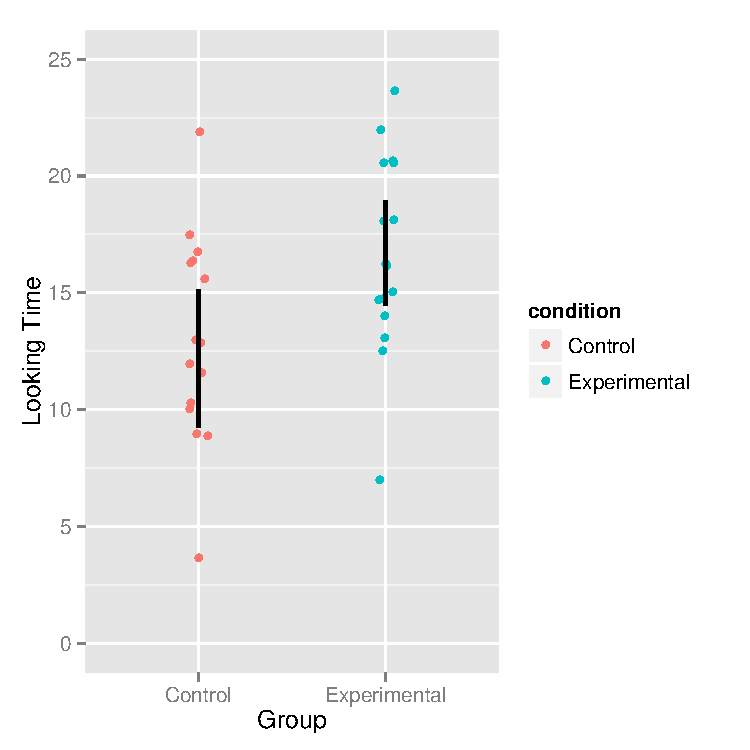
\includegraphics[width=2.5in]{../plots/scatter.pdf}
	\caption{\label{fig:plots}....}
\end{figure}

The most conventional visualization used in infancy research is the standard ``dynamite'' bar plot, with error bars representing the standard error of the mean. While they are clear and easy to read, these plots are relatively uninformative from the perspective of revealing features of the underlying dataset, as has been noted extensively in other literatures \cite{plosbio}. Authors should strongly consider moving towards plotting the individual participants' 

In addition, the use of the standard error of the mean (SEM) is potentially misleading as it does not provide a good guide for inference. First, researchers should move from SEM to 95\% confidence intervals \cite{cumming2013}. Second, researchers are often taught that non-overlapping standard errors are a meaningful indicator of the outcome of a statistical test---this is in fact false \cite{cumming2006}. Such rules of thumb are doubly misleading when within-subject means are plotted side-by-side, since the appropriate statistical test is paired---hence SEM and CI are not inferentially relevant. 

\paragraph{Post-hoc analyses}

Although such analyses are interesting, they are inevitably underpowered 

\paragraph{Multi-trial paradigms}


\section{Conclusions: Implications for a literature}

\bibliographystyle{apacite}
\bibliography{methods}

\end{document}